%\chapter{Paquímetro}

\section{Objetivos}

\begin{itemize}
\item Conhecimento do paquímetro e familiarização com seu uso.
\end{itemize}

\section{Material}

\setlist[1]{itemsep=-5pt}
\begin{multicols}{3}
\begin{itemize}
\item Paquímetro
\item Cilindro
\item Tarugo
\item Peça com furo cego
\item Régua
\item Tiras de papel
\end{itemize}
\end{multicols}

\section{Fundamentos}
O paquímetro, também conhecido como calibre, é um instrumento de precisão muito usado em oficinas e laboratórios para: medidas de comprimentos, diâmetros de tarugos, diâmetro interno e externo de tubos, profundidades de furos, transformação de polegadas em milímetros e vice-versa. A peça mais importante do paquímetro é o nônio, a qual merece um estudo à parte.

\begin{figure}[ht]
\centering
\label{fig:paq}
\includegraphics[scale=0.2]{figuras/paqx.png} 
\caption{Paquímetro}
\end{figure}

\setlist[1]{itemsep=-5pt}
\begin{multicols}{2}
\begin{enumerate}
\item Orelha fixa
\item Orelha móvel
\item Nônio ou vernier (polegada)
\item Parafuso de trava
\item Cursor
\item Escala fixa de polegadas
\item Bico fixo
\item Encosto fixo
\item Encosto móvel
\item Bico móvel
\item Nônio ou vernier (milímetro)
\item Impulsor
\item Escala fixa de milímetro
\item Haste de profundidade
\end{enumerate}
\end{multicols}

\subsection{Nônio}
\emph{Nônio} é uma pequena régua cujas características determinam o grau de precisão do paquímetro. O nônio permite fazer, com exatidão, leituras de frações de milímetro. Pode ser construído com uma precisão maior ou menor, como  $\frac{1}{10}mm$, $\frac{1}{50}mm$ e até  $\frac{1}{100}mm$. O princípio da construção do nônio é basicamente o seguinte: ``x'' milímetos da régua principal constituem o seu comprimento, o qual é dividido em ``n'' partes.


\begin{figure}[ht]
\label{fig:nonio}
\centering
\begin{minipage}{\linewidth}
\begin{minipage}{0.4\linewidth}
\includegraphics[scale=0.2]{figuras/nonio1.png} 
\end{minipage}
\begin{minipage}{0.4\linewidth}
\includegraphics[scale=0.2]{figuras/nonio2.png} 
\end{minipage}
\end{minipage}
\caption{Nônio}
\end{figure}

No caso da Figura \ref{fig:nonio}, o comprimento do nônio é $9mm$ e foi dividido em 10 partes iguais. Portanto, cada divisão desse nônio é igual a $9/10mm$. Se o traço 0(zero) do nônio está em coincidência com o traço 0 da régua, isto significa que o traço 1 do nônio está afastado $1/10$ do traço de $1mm$ da régua. Por outro lado, se o traço 1 do nônio coincidisse com o traço $1mm$ da régua, o nônio teria sido deslocado $1/10mm$. O mesmo raciocínio é válido para os demais traços, como por exemplo: no caso de o traço 6 do nônio coincidir com o traço de $6mm$ da régua, é porque houve um deslocamento do nônio equivalente a $6/10mm$.

\textsc{\textbf{Precisão do Nônio}} - Para encontrar o grau de precisão de um nônio:
\begin{enumerate}
\item Mede-se o comprimento (L) do nônio (a distância entre o primeiro e o último traço);
\item Divide-se o comprimento (L) por (n), que é o número de divisões do nônio;
\item Sutrai-se o resultado do número inteiro de milímetro imediatamente superior.
\end{enumerate}


Para o Nônio da Figura \ref{fig:reg-non}, temos:
\begin{enumerate}
\item $L = 9mm$;
\item $n=10; 9mm\div 10= 0,9mm$;
\item Precisão = $1mm - 0,9mm = 0,1mm = 1/10mm$.
\end{enumerate}

\textsc{\textbf{Medindo com o Paquímetro}}:
\begin{enumerate}
\item Encoste a peça a medir na mandíbula fixa;
\item Com o polegar no impulsor, desloque o mandíbula móvel até que ela encoste suavemente na outra extremidade da peça;
\item Leia na régua principal o número de milímetros inteiros, ou seja, os que estão à esquerda do zero do nônio;
\item Para a leitura da fração de milímetros, veja qual o traço do nônio que coincide com \textsc{qualquer} traço da régua principal, e multiplique o número desse traço pela precisão;
\item A figura abaixo dá uma ideia de como utilizar as diversas parte do paquímetro.

\end{enumerate}

\begin{figure}[ht]
\centering
\label{fig:uso-paq}
\includegraphics[scale=0.2]{figuras/uso-paq.png} 
\caption{Uso do paquímetro}
\end{figure}

XXXXXXXXXXXXXXXXXXXXXXX
XXXXXXXXXXXXXXXXXXXXXXX

\section{Pré-laboratório}
Determine a precisão do nônio ilustrado abaixo e faça as leituras das figuras subsequentes.

\begin{figure}[ht]
\label{fig:reg-non}
\centering
\begin{minipage}{\linewidth}
\begin{minipage}{0.4\linewidth}
\includegraphics[scale=0.2]{figuras/ex1.png} 
\end{minipage}
\begin{minipage}{0.4\linewidth}
\includegraphics[scale=0.2]{figuras/ex2.png} 
\end{minipage}

\begin{minipage}{0.4\linewidth}
Leitura:\rule{3cm}{0.4pt}
\end{minipage}
\begin{minipage}{0.4\linewidth}
Leitura:\rule{3cm}{0.4pt}
\end{minipage}

\begin{minipage}{0.4\linewidth}
\includegraphics[scale=0.2]{figuras/ex3.png} 
\end{minipage}
\begin{minipage}{0.4\linewidth}
\includegraphics[scale=0.2]{figuras/ex4.png} 
\end{minipage}
\end{minipage}
\end{figure}

% % % % % % % % % % % % % % % % % %
\def\esqnonio{-0.1cm}
\def\largnonio{12*0.19cm}

\begin{minipage}{\linewidth}
\begin{minipage}{0.4\linewidth}

%\begin{tikzpicture}[y=.2cm, x=0.05*\textwidth,font=\sffamily]
\begin{tikzpicture}
%régua
    \draw (0,0) -- (3cm,0);
    
    \foreach \x in {0,...,2}
        \draw (\x*1cm,0pt) -- (\x*1cm,15pt)
        node[anchor=south] {$\x$};

    \foreach \x in {1,...,29}
        \draw (\x*0.1cm,0pt) -- (\x*0.1cm,5pt)
        node[anchor=south] {};

    \foreach \x in {1,3,5}
        \draw (\x*0.5cm,0pt) -- (\x*0.5cm,10pt)
        node[anchor=south] {};

%Nônio
	\draw [gray, ultra thick, fill=lightgray] (\esqnonio, -0.02cm) rectangle (\esqnonio + \largnonio,-0.5cm);
      
    \foreach \x in {0,...,10}
        \draw (\x*0.19cm, -0.01cm) -- (\x*0.19cm, -0.15cm)
        node[anchor=north] {{\tiny \x}};

    \foreach \x in {0,...,9}
        \draw (\x*0.19cm + 0.095cm, -0.01cm) -- (\x*0.19cm + 0.095cm, -0.10cm)
        node[anchor=south] {};
        
	\draw [fill] (0*0.19cm , -0.15cm) circle (0.02);
    
\end{tikzpicture}
\\

Precisão:\rule{3cm}{0.4pt}
\\
\vspace{1cm}

\end{minipage}
\begin{minipage}{0.4\linewidth}

\def\esqnonio{0.43cm}
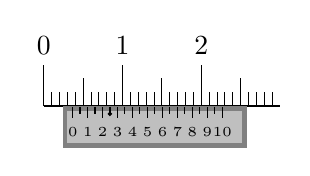
\begin{tikzpicture}
%régua
    \draw (0,0) -- (3cm,0);
    
    \foreach \x in {0,...,2}
        \draw (\x*1cm,0pt) -- (\x*1cm,15pt)
        node[anchor=south] {$\x$};

    \foreach \x in {1,...,29}
        \draw (\x*0.1cm,0pt) -- (\x*0.1cm,5pt)
        node[anchor=south] {};

    \foreach \x in {1,3,5}
        \draw (\x*0.5cm,0pt) -- (\x*0.5cm,10pt)
        node[anchor=south] {};

%Nônio
	\draw [gray, ultra thick, fill=lightgray] (\esqnonio, -0.03cm) rectangle (\esqnonio + \largnonio,-0.5cm);
      
    \foreach \x in {0,...,10}
        \draw (\esqnonio + 0.0975cm + \x*0.19cm, -0.01cm) -- (\esqnonio + 0.0975cm + \x*0.19cm, -0.15cm)
        node[anchor=north] {{\tiny \x}};

    \foreach \x in {0,...,9}
        \draw (\esqnonio + 0.095cm + \x*0.19cm + 0.095cm, -0.01cm) -- (\esqnonio + 0.095cm + \x*0.19cm + 0.095cm, -0.10cm)
        node[anchor=south] {};

	\draw [fill] (\esqnonio + 0.095cm + 2.5*0.19cm, -0.10cm) circle (0.02);

\end{tikzpicture}
\\

Precisão:\rule{3cm}{0.4pt}
\\
\vspace{1cm}
\end{minipage}
\begin{minipage}{0.4\linewidth}

\def\esqnonio{0.59cm}
\begin{tikzpicture}
%régua
    \draw (0,0) -- (3cm,0);
    
    \foreach \x in {0,...,2}
    	\def\y{\x + 13}
        \draw (\x*1cm,0pt) -- (\x*1cm,15pt)
        node[anchor=south] {$\directlua{tex.print(\y);}$};

    \foreach \x in {1,...,29}
        \draw (\x*0.1cm,0pt) -- (\x*0.1cm,5pt)
        node[anchor=south] {};

    \foreach \x in {1,3,5}
        \draw (\x*0.5cm,0pt) -- (\x*0.5cm,10pt)
        node[anchor=south] {};

%Nônio
	\draw [gray, ultra thick, fill=lightgray] (\esqnonio, -0.03cm) rectangle (\esqnonio + \largnonio,-0.5cm);
      
    \foreach \x in {0,...,10}
        \draw (\esqnonio + 0.0975cm + \x*0.19cm, -0.01cm) -- (\esqnonio + 0.0975cm + \x*0.19cm, -0.15cm)
        node[anchor=north] {{\tiny \x}};

    \foreach \x in {0,...,9}
        \draw (\esqnonio + 0.095cm + \x*0.19cm + 0.095cm, -0.01cm) -- (\esqnonio + 0.095cm + \x*0.19cm + 0.095cm, -0.10cm)
        node[anchor=south] {};

	\draw [fill] (\esqnonio + 0.095cm + 8.5*0.19cm, -0.10cm) circle (0.02);

\end{tikzpicture}
\\

Precisão:\rule{3cm}{0.4pt}
\\
\vspace{1cm}

\end{minipage}
\begin{minipage}{0.4\linewidth}

\def\esqnonio{0.27cm}
\begin{tikzpicture}
%régua
    \draw (0,0) -- (3cm,0);
    
    \foreach \x in {0,...,2}
    	\def\y{\x + 13}
        \draw (\x*1cm,0pt) -- (\x*1cm,15pt)
        node[anchor=south] {$\directlua{tex.print(\y);}$};

    \foreach \x in {1,...,29}
        \draw (\x*0.1cm,0pt) -- (\x*0.1cm,5pt)
        node[anchor=south] {};

    \foreach \x in {1,3,5}
        \draw (\x*0.5cm,0pt) -- (\x*0.5cm,10pt)
        node[anchor=south] {};

%Nônio
	\draw [gray, ultra thick, fill=lightgray] (\esqnonio, -0.03cm) rectangle (\esqnonio + \largnonio,-0.5cm);
      
    \foreach \x in {0,...,10}
        \draw (\esqnonio + 0.0975cm + \x*0.19cm, -0.01cm) -- (\esqnonio + 0.0975cm + \x*0.19cm, -0.15cm)
        node[anchor=north] {{\tiny \x}};

    \foreach \x in {0,...,9}
        \draw (\esqnonio + 0.095cm + \x*0.19cm + 0.095cm, -0.01cm) -- (\esqnonio + 0.095cm + \x*0.19cm + 0.095cm, -0.10cm)
        node[anchor=south] {};

	\draw [fill] (\esqnonio + 0.095cm + 6.5*0.19cm, -0.10cm) circle (0.02);

\end{tikzpicture}
\\

Precisão:\rule{3cm}{0.4pt}

\vspace{1cm}
\end{minipage}
\begin{minipage}{0.4\linewidth}

\def\esqnonio{0.27cm}
\begin{tikzpicture}
%régua
    \draw (0,0) -- (3cm,0);
    
    \foreach \x in {0,...,2}
    	\def\y{\x + 13}
        \draw (\x*1cm,0pt) -- (\x*1cm,15pt)
        node[anchor=south] {$\directlua{tex.print(\y);}$};

    \foreach \x in {1,...,29}
        \draw (\x*0.1cm,0pt) -- (\x*0.1cm,5pt)
        node[anchor=south] {};

    \foreach \x in {1,3,5}
        \draw (\x*0.5cm,0pt) -- (\x*0.5cm,10pt)
        node[anchor=south] {};

%Nônio
	\draw [gray, ultra thick, fill=lightgray] (\esqnonio, -0.03cm) rectangle (\esqnonio + \largnonio,-0.5cm);
      
    \foreach \x in {0,...,10}
        \draw (\esqnonio + 0.0975cm + \x*0.19cm, -0.01cm) -- (\esqnonio + 0.0975cm + \x*0.19cm, -0.15cm)
        node[anchor=north] {{\tiny \x}};

    \foreach \x in {0,...,9}
        \draw (\esqnonio + 0.095cm + \x*0.19cm + 0.095cm, -0.01cm) -- (\esqnonio + 0.095cm + \x*0.19cm + 0.095cm, -0.10cm)
        node[anchor=south] {};

	\draw [fill] (\esqnonio + 0.095cm + 6.5*0.19cm, -0.10cm) circle (0.02);

\end{tikzpicture}
\\

Precisão:\rule{3cm}{0.4pt}
\end{minipage}
\end{minipage}

\section{Procedimento}
Obs:Antes de você fazer esta prática é conveniente conhecer o conteúdo do texto sobre \emph{Algarismos Significativos}. O aluno que não observar as regras sobre Algarismos Significativos em seus relatórios será penalizado.

\subsection{Cálculos de volumes e diâmetros}
Utilizando o cálculo do \emph{valor médio},em que o número de termos  é o mesmo dos números componentes da equipe, como uso do paquímetro, determine:

\subsubsection{O volume da peça cilíndrica maior} 
\begin{table}[h]
\centering
\begin{tabular}{|l|*{4}{c|}}
\hline & Medida& Medida& Medida& Medida \\
\hline Diâmetro(mm)& & &  & \\ 
\hline Altura(mm)& & &  & \\ 
\hline
\end{tabular}

\end{table}

\begin{table}[h]
\centering
\begin{tabular}{|p{10cm}|}
\hline Cálulo do Volume \\ 
\\
\\
\hline
\end{tabular}
\end{table}

\subsubsection{O diâmetro do tarugo} 
\begin{table}[h]
\centering
\begin{tabular}{|l|*{4}{c|}}
\hline & Medida& Medida& Medida& Medida \\
\hline Diâmetro(mm)& & &  & \\ 
\hline
\end{tabular}

\end{table}

\subsubsection{O volume de ferro da peça com furo cego} 

\begin{table}[ht]
\centering
\begin{tabular}{|l|*{4}{c|}}
\hline & Medida& Medida& Medida& Medida \\
\hline Diâmetro externo(mm)& & &  & \\ 
\hline Altura externa(mm)& & &  & \\ 
\hline Diâmetro interno(mm)& & &  & \\ 
\hline Altura interna(mm)& & &  & \\ 
\hline
\end{tabular}

\end{table}

\begin{table}[h]
\centering
\begin{tabular}{|p{10cm}|}
\hline Cálulo do Volume \\ 
\\
\\
\hline
\end{tabular}
\end{table}

\subsection{Outros cálculos}
Com o auxílio de tiras de papel, envolva as peças e, com uma régua, meça os comprimentos das circunferências externas. Anote somente os valores obtido por você.

\begin{table}[h]
\centering
\begin{tabular}{|p{10cm}|}
\hline 
\\
\\
\hline
\end{tabular}
\end{table}

\section{Questionário}
\begin{enumerate}
\item A partir dos valores médios dos diâmetros obtido com o paquímetro, determine o comprimento da circunferência externa das três peças.
\item Considere os valores dos comprimentos das circunferências obtidas com o paquímetro e com uma régua, quais os de maior precisão?
\item Nas medidas feitas na peça como o furo cego, para o cálculo do volume, quais as que podem contribuir no mesmo resultado com maior erro? Por quê?
\item Qual a menor fração de milímetro que pode ser lida com o paquímetro que você utilizou?
\item Qual a precisão de um paquímetro cujo nônio tem $49mm$ de comprimento e está dividido em 50 partes iguais?
\item O nônio de um paquímetro tem $29mm$ de comprimento. A precisão do mesmo é de $0,1mm$. En quantas partes foi dividido o nônio?
\item Num paquímetro de $0,05mm$ de sensibilidade, a distância  entre o zero da escala e o zero do vernier é de $11,5cm$, sendo que o 13º traço do vernier coincidiu. Qual o valor da medida?
\item Qual seria a leitura acima se a sensibilidade fosse $0,02mm$?
\end{enumerate}

